\documentclass[11pt,a4paper]{article}
\usepackage[margin=1in]{geometry}
\usepackage{amsmath,amssymb,amsfonts}
\usepackage{graphicx}
\usepackage{booktabs}
\usepackage{longtable}
\usepackage{tabularx}
\usepackage{array}
\usepackage{float}
\usepackage{cite}
\usepackage{hyperref}
\usepackage{microtype}

\hypersetup{
    colorlinks=true,
    linkcolor=blue,
    citecolor=blue,
    urlcolor=blue
}

\title{\textbf{Automated Quantitative Surface Grain Density and Internal Macroporosity Retrieval for Main-Belt and Near-Earth Asteroids}}

\author{Aidan Gray \\ Stuyvesant High School \\ aidangray42@gmail.com}
\date{\today}

\begin{document}

\maketitle

\begin{abstract}
Determining the surface mineralogy, bulk grain density, and internal structure of minor bodies is fundamental to understanding solar system formation, parent body differentiation, and planetary defense hazards. However, deriving physical properties from disk-integrated visible and near-infrared (VNIR; $0.4$--$2.5\,\mu\text{m}$) reflectance spectra remains severely hindered by non-linear multiple scattering, space weathering, photometric phase reddening, and mineral endmember collinearity. We present an automated computational framework for spectral unmixing, grain density inversion, and macroporosity retrieval. The engine converts directional-hemispherical reflectance to Hapke Single Scattering Albedo (SSA) space, normalizes phase reddening via an albedo-dependent sigmoidal model, and removes NEATM thermal infrared contamination. Non-negative mineral abundances are optimized using Sequential Least Squares Programming (SLSQP) bounded by Pseudo-Huber loss and an adaptive $L_1$ LASSO sparsity penalty. Automatically selecting between Stony/Metallic and Primitive/Aqueous endmember libraries using the Akaike Information Criterion (AIC), surface cross-sectional area fractions are mapped to mass fractions to compute crustal grain densities ($\rho_{\text{grain}}$). Combining derived grain densities with validated bulk density measurements ($\rho_{\text{bulk}}$) yields internal macroporosities ($\Phi$). Uncertainties are propagated through 150 Monte Carlo realizations using a Lag-1 Autoregressive $AR(1)$ noise model ($\phi = 0.65$) to account for inter-channel correlations. Applied across 266 asteroid spectra ($139$ meeting quality criteria), the pipeline achieved a mean reduced chi-squared fit of $\chi^2_{\text{red}} = 0.961$ ($0.983$ for Stony targets; $0.834$ for Primitive targets). Stony asteroids yielded a mean grain density of $\bar{\rho}_{\text{grain}} = 4.11 \pm 0.17\,\text{g/cm}^3$, whereas featureless carbonaceous targets converged on a baseline prior ($\bar{\rho}_{\text{grain}} = 2.358 \pm 0.002\,\text{g/cm}^3$). Benchmark retrievals against spacecraft and laboratory reference targets—including 4 Vesta ($\rho_{\text{grain}} = 4.10 \pm 0.05\,\text{g/cm}^3$, $\Phi = 15.5\%$), 433 Eros ($\rho_{\text{grain}} = 4.49 \pm 0.11\,\text{g/cm}^3$, $\Phi = 34.1\%$), and 24 Themis ($\rho_{\text{grain}} = 2.36 \pm 0.005\,\text{g/cm}^3$, $\Phi = 23.2\%$)—demonstrate that this automated approach reliably bridges remote sensing observations and in-situ planetary exploration.
\end{abstract}

\newpage

\section{Introduction}
Reflectance spectroscopy in the visible and near-infrared (VNIR; $0.40$--$2.50\,\mu\text{m}$) spectrum provides the primary observational basis for inferring the surface composition and evolutionary history of main-belt and near-earth asteroids \cite{DeMeo2009, Gaffey1993}. However, transforming telescopic reflectance spectra into quantitative mineral abundances and physical bulk parameters poses severe inverse mathematical challenges \cite{Tarantola2005, Hapke1981}. Photon scattering within planetary regoliths is inherently non-linear due to multiple inter-particle reflections \cite{Hapke1981, Hapke2012}. Furthermore, observations are degraded by space weathering continuum steepening ($npFe^0$) \cite{Hapke2001, Pieters2000}, phase reddening at elevated solar phase angles \cite{Sanchez2012, Fornasier2015}, and thermal infrared re-radiation at wavelengths $> 1.8\,\mu\text{m}$ \cite{Harris1998}.

To address these coupled inverse problems, we developed an automated computational framework \cite{Tarantola2005, Hapke1981, Consolmagno2008, Carry2012}. The pipeline transforms observed reflectance spectra into Single Scattering Albedo (SSA) space via Hapke radiative transfer theory \cite{Hapke1981, Hapke2012}, dynamically normalizes photometric phase reddening using a sigmoidal function scaled to geometric albedo \cite{Sanchez2012, Fornasier2015}, removes thermal emission components using the Near-Earth Asteroid Thermal Model (NEATM) \cite{Harris1998}, and optimizes mineral modal abundances via Sequential Least Squares Programming (SLSQP) bounded by a robust Pseudo-Huber loss function \cite{Lawson1995, Huber1964, Bioucas2012}. For unclassified targets, candidate fits from Stony and Primitive spectral libraries are automatically evaluated using the Akaike Information Criterion (AIC) to prevent over-parameterization \cite{Akaike1974}.

The retrieved area fractions are mapped to mass fractions and inverted via mass-weighted harmonic summation to compute surface grain densities ($\rho_{\text{grain}}$) \cite{Consolmagno2008, Britt2003}. Combining these values with validated bulk density measurements ($\rho_{\text{bulk}}$) yields accurate estimates of internal macroporosity ($\Phi$), while filtering out non-physical placeholder bulk density tags \cite{Carry2012}. Uncertainties are propagated through 150 Monte Carlo iterations employing a Lag-1 autoregressive noise model to account for inter-channel spectral correlations \cite{Efron1993, Press2007}. Applied across 266 asteroid spectra ($139$ meeting quality filters), the framework achieved an overall mean reduced chi-squared fit of $\chi^2_{\text{red}} = 0.961$ ($0.983$ across silicate-rich Stony targets; $0.834$ across featureless Primitive continua). Surface grain densities inverted across diagnostic Stony targets averaged $\bar{\rho}_{\text{grain}} = 4.11 \pm 0.17\,\text{g/cm}^3$, whereas featureless carbonaceous continua converged on an IOM/serpentine baseline prior ($\bar{\rho}_{\text{grain}} \approx 2.36\,\text{g/cm}^3$). Benchmark evaluations against spacecraft-characterized and ground-based spectroscopic reference targets—including 4 Vesta ($\rho_{\text{grain}} = 4.10 \pm 0.05\,\text{g/cm}^3$; Dawn) \cite{Russell2012}, 433 Eros ($\rho_{\text{grain}} = 4.49 \pm 0.11\,\text{g/cm}^3$; NEAR Shoemaker) \cite{Veverka2001}, and 24 Themis ($\rho_{\text{grain}} = 2.36 \pm 0.005\,\text{g/cm}^3$; IRTF spectroscopy) \cite{Campins2010}—demonstrate that this automated approach reliably bridges telescopic observations and in-situ planetary exploration \cite{DeMeo2009, Britt2002, Lauretta2019, Watanabe2019}.

This pipeline eliminates the need for manual curve-fitting by combining physical constraints with automated spectral unmixing, grain density inversion, and macroporosity estimation \cite{Tarantola2005, Consolmagno2008, Carry2012}. By coupling Hapke radiative transfer theory \cite{Hapke1981, Hapke2012}, NEATM thermal corrections \cite{Harris1998}, Pseudo-Huber loss optimization \cite{Huber1964}, and information-theoretic model selection \cite{Akaike1974}, this engine enables high-throughput, reproducible physical characterization across large astronomical databases, directly supporting planetary defense, resource prospecting, and nebular condensation models \cite{DeMeo2009, Britt2002, Lauretta2019, Watanabe2019}.

\section{Theoretical Methods and Physical Formulation}

\subsection{Hapke Single Scattering Albedo (SSA) Transformation}
Reflectance spectra measured at disk-integrated geometries do not combine linearly in reflectance space because photons undergo multiple internal scatterings within adjacent regolith grains \cite{Hapke1981}. Following Hapke (1981, 2012), directional-hemispherical reflectance $R(\lambda)$ is converted into Single Scattering Albedo $w(\lambda)$ using the isotropic scattering approximation:
\begin{equation}
w(\lambda) = 1 - \left[ \frac{1 - R(\lambda)}{1 + 2R(\lambda)} \right]^2
\label{eq:hapke_ssa}
\end{equation}
In SSA space, photon scattering cross-sections combine linearly as a weighted sum of endmember SSA spectra $w_j(\lambda)$ \cite{Hapke1981, Hapke2012}:
\begin{equation}
w_{\text{model}}(\lambda) = \sum_{j=1}^{M} f_j w_j(\lambda)
\label{eq:ssa_linear}
\end{equation}
where $f_j$ denotes the surface cross-sectional area fraction of endmember $j$, subject to non-negativity ($f_j \ge 0$) and unit sum ($\sum f_j = 1.0$) constraints \cite{Lawson1995}.

\subsection{Dynamic Photometric Phase Reddening Normalization}
At solar phase angles $\alpha > 5^\circ$, single-scattering phase functions and micro-shadowing induce systemic continuum reddening \cite{Sanchez2012, Fornasier2015}. The pipeline computes a continuous, albedo-dependent phase reddening coefficient $k_{\text{phase}}(A)$ ($\mu\text{m}^{-1}/\text{deg}$) scaled to visual geometric albedo $A$:
\begin{equation}
k_{\text{phase}}(A) = 0.00012 + \frac{0.00048}{1 + \exp\left[-18.0 \cdot (A - 0.09)\right]}
\label{eq:phase_reddening}
\end{equation}
The spectrum is normalized back to standard $5^\circ$ geometry via:
\begin{equation}
R_{\text{corr}}(\lambda) = R(\lambda) \cdot \exp\left[ -k_{\text{phase}}(A) \cdot (\alpha - 5.0) \cdot (\lambda - 0.55) \right]
\label{eq:phase_correction}
\end{equation}

\subsection{NEATM Thermal Emission Weighting and Atmospheric Tellurics}
Near-Earth and main-belt asteroids observed at small heliocentric distances $r_{\text{h}}$ exhibit thermal tail re-radiation at $\lambda > 1.8\,\mu\text{m}$ \cite{Harris1998}. The pipeline calculates the subsolar equilibrium temperature $T_{\text{ss}}$ using the Near-Earth Asteroid Thermal Model (NEATM) \cite{Harris1998}:
\begin{equation}
T_{\text{ss}} = \left[ \frac{(1 - A) S_0}{\eta \epsilon \sigma r_{\text{h}}^2} \right]^{1/4}
\label{eq:neatm_temp}
\end{equation}
where $S_0 = 1361\,\text{W/m}^2$, $\eta = 1.20$ is the beaming factor, $\epsilon = 0.90$ is infrared emissivity, and $\sigma$ is the Stefan-Boltzmann constant. When $T_{\text{ss}} > 280\,\text{K}$, channel weighting factors $W(\lambda)$ dynamically attenuate thermal contamination:
\begin{equation}
W(\lambda) = \frac{1}{1 + 0.8 \cdot (T_{\text{ss}}/300)^4 \cdot \max(0, \lambda - 1.8)^2}
\label{eq:thermal_weights}
\end{equation}
Channels corresponding to atmospheric telluric water absorption bands ($1.35$--$1.42\,\mu\text{m}$ and $1.80$--$1.92\,\mu\text{m}$) are assigned $W(\lambda) = 0.50$ \cite{DeMeo2009}.

\subsection{Space Weathering Compensation}
Nanophase iron particles ($npFe^0$) produced by micrometeorite bombardment and solar wind irradiation darken absorption bands and steepen continuum slopes \cite{Hapke2001, Pieters2000}. Because linear additive mixing holds strictly in SSA space, space weathering slope compensation $C_{\text{sw}}(\lambda) = \exp[-S(\lambda - 0.55)]$ is applied directly in SSA space as an empirical continuum correction \cite{Hapke2001, Bioucas2012}:
\begin{equation}
w_{\text{model}}(\lambda) = \exp\left[-S(\lambda - 0.55)\right] \cdot \left( \sum_{j=1}^{M} f_j w_j(\lambda) \right)
\label{eq:weathering_ssa}
\end{equation}
where $S \in [-0.15, 1.50]$ is the optimized space weathering slope factor \cite{Hapke2001}. Modeling weathering as an SSA-space continuum correction preserves objective function convexity during Sequential Least Squares Programming (SLSQP) \cite{Lawson1995}.

\subsection{Robust SLSQP Optimization with Multi-Start Pseudo-Huber Loss}
Spectral unmixing solves for abundance vector $\vec{f}$ and weathering slope $S$ using SLSQP optimization \cite{Lawson1995}. Abundances are strictly constrained to be non-negative and sum to unity ($\sum f_j = 1.0$) \cite{Lawson1995, Bioucas2012}. To prevent outlier channels from skewing the fit, the pipeline replaces standard $L_2$ squared loss with the smooth Pseudo-Huber loss function ($\delta = 0.005$) \cite{Huber1964, Press2007}:
\begin{equation}
\mathcal{L}_{\text{Huber}}(r_i) = \delta^2 \left( \sqrt{1 + (r_i / \delta)^2} - 1 \right)
\label{eq:pseudo_huber}
\end{equation}
where $r_i = w_{\text{model}}(\lambda_i) - w_{\text{obs}}(\lambda_i)$. Because the joint optimization over abundance vector $\vec{f}$ and weathering slope $S$ in Equation~\ref{eq:weathering_ssa} is non-convex, the optimizer executes multi-start SLSQP searches across a initialized grid of weathering slopes $S \in [-0.05, 0.60]$ to guarantee global minimum convergence \cite{Lawson1995}.

\subsection{Mass-Weighted Harmonic Grain Density Inversion and Macroporosity}
Surface cross-sectional area fractions $f_j$ map directly to volume fractions $V_j / V_{\text{total}}$ in fine-grained regoliths \cite{Hapke1981, Consolmagno2008}. To rigorously compute the pore-free grain density $\rho_{\text{grain}}$, area fractions $f_j$ are mapped to mass fractions $w_j$ via $w_j = \frac{f_j \rho_j}{\sum_{k} f_k \rho_k}$ \cite{Consolmagno2008, Britt2003}. Mass-weighted harmonic summation then yields:
\begin{equation}
\rho_{\text{grain}} = \left[ \sum_{j=1}^{M} \frac{w_j}{\rho_j} \right]^{-1} = \sum_{j=1}^{M} f_j \rho_j
\label{eq:harmonic_density}
\end{equation}
where $\rho_j$ is the pure mineral crystal density of endmember $j$.

When an authentic, measured bulk density $\rho_{\text{bulk}}$ is available from spacecraft tracking or double-star mutual occultations \cite{Carry2012}, internal macroporosity $\Phi$ is calculated directly as \cite{Consolmagno2008, Carry2012}:
\begin{equation}
\Phi = 1 - \frac{\rho_{\text{bulk}}}{\rho_{\text{grain}}}
\label{eq:macroporosity}
\end{equation}
Targets tagged with unverified placeholder bulk densities (e.g., NEOWISE default estimates) are explicitly flagged as `Not Calculated' to prevent invalid structural inferences \cite{Carry2012}.

\subsection{Autocorrelated $AR(1)$ Monte Carlo Uncertainty Propagation}
To rigorously quantify uncertainties across all derived parameters—including modal mineral abundances $f_j$, grain density $\rho_{\text{grain}}$, and macroporosity $\Phi$—a single, integrated stochastic error propagation framework is established \cite{Efron1993, Press2007}. Rather than assuming independent channel errors, observational noise is modeled using a Lag-1 Autoregressive process $AR(1)$ to preserve the inter-channel correlations typical of CCD and NIR array spectrometers \cite{Efron1993, Press2007}:
\begin{equation}
\epsilon_i^{(k)} = \phi \cdot \epsilon_{i-1}^{(k)} + \sqrt{1 - \phi^2} \cdot \eta_i^{(k)}, \quad \eta_i^{(k)} \sim \mathcal{N}\left(0, [\sigma_{\text{obs}}(\lambda_i)]^2\right)
\label{eq:ar1_noise}
\end{equation}
where $\phi = 0.65$ represents the channel correlation coefficient, and $\eta_i^{(k)}$ is drawn from a zero-mean normal distribution scaled to local channel standard deviation \cite{Efron1993, Press2007}.

For each synthetic realization $k$, the full non-linear inversion pipeline—comprising SSA transformation, phase reddening correction, NEATM subtraction, and constrained SLSQP optimization—is executed from initial pre-processing through final parameter derivation \cite{Hapke1981, Lawson1995, Huber1964}. This produces $K$ independent solutions for mineral fractions $f_j^{(k)}$, grain density $\rho_{\text{grain}}^{(k)}$, and macroporosity $\Phi^{(k)}$ \cite{Consolmagno2008, Carry2012}.

\section{Methodological Justifications}
The computational pipeline coordinates end-to-end data ingestion, preprocessing, optimization, and Monte Carlo uncertainty quantification \cite{Tarantola2005, Press2007}. Below is an exhaustive comparative breakdown detailing why specific numerical methods were chosen over competing alternatives \cite{Lawson1995, Huber1964, Akaike1974}.

\subsection{Sequential Least Squares Programming with Pseudo-Huber Loss}
Ordinary Least Squares (OLS) permits negative abundances, violating physics \cite{Lawson1995}. Standard $L_2$ loss is highly sensitive to cosmic rays and calibration spikes \cite{Huber1964, Press2007}. Pseudo-Huber loss was selected because it behaves like $L_2$ loss for small residuals while transitioning to linear $L_1$ loss for outliers, providing outlier immunity \cite{Huber1964, Press2007}.

The objective function must be continuous and convex within bounded constraints \cite{Lawson1995, Huber1964}.

\subsection{AIC Model Selection and AR(1) Noise Propagation}
AIC model selection prevents over-fitting by penalizing unnecessary endmembers when choosing between candidate mineral libraries \cite{Akaike1974}. Simple linear arithmetic averaging of grain densities is physically incorrect because volume and mass fractions combine harmonically \cite{Consolmagno2008, Britt2003}. Independent identically distributed (i.i.d.) Gaussian noise bootstrapping was rejected because adjacent spectrometer channels exhibit strong correlation \cite{Efron1993, Press2007}. An $AR(1)$ Lag-1 autoregressive noise model was selected to simulate realistic, channel-correlated noise realizations \cite{Efron1993, Press2007}.

\section{Endmember Spectral Libraries and Mineralogical Rationale}
\label{sec:libraries}

Spectral endmember libraries were constructed using reference samples from the USGS \texttt{splib07a} \cite{Clark2007} and NASA RELAB databases \cite{Pieters2004}, with grain densities compiled from physical geochemistry literature \cite{Consolmagno2008, Deer2013, Buchwald1975, Britt2003, Macke2011}. Tables~\ref{tab:stony_library} and \ref{tab:primitive_library} outline library specifications.

\begin{table}[H]
\centering
\caption{\textbf{Stony and Metallic Sub-Library Endmember Specifications.}}
\label{tab:stony_library}
\small
\begin{tabularx}{\textwidth}{p{0.28\textwidth} p{0.32\textwidth} c c p{0.18\textwidth}}
\toprule
Mineral Name & Chemical Formula / Description & $\rho_{\text{grain}}$ & $\sigma_{\rho}$ & Database Source \\
\midrule
Olivine\_Fo90\_Mg & Forsterite rich $(\text{Mg}_{0.90}\text{Fe}_{0.10})_2\text{SiO}_4$ & 3.32\cite{Consolmagno2008} & 0.02\cite{Consolmagno2008} & USGS \texttt{splib07a}\cite{Clark2007} \\
Olivine\_Fa50\_Fe & Fayalite rich $(\text{Mg}_{0.50}\text{Fe}_{0.50})_2\text{SiO}_4$ & 3.84\cite{Consolmagno2008} & 0.04\cite{Consolmagno2008} & RELAB \texttt{c1ol02}\cite{Pieters2004} \\
Orthopyroxene\_En86 & Enstatite $(\text{Mg}_{0.86}\text{Fe}_{0.14})\text{SiO}_3$ & 3.28\cite{Consolmagno2008} & 0.02\cite{Consolmagno2008} & RELAB \texttt{c1pp01}\cite{Pieters2004} \\
Pigeonite\_LowCa & Monoclinic pyroxene solid solution & 3.40\cite{Consolmagno2008} & 0.03\cite{Consolmagno2008} & RELAB \texttt{c1px}\cite{Pieters2004} \\
Clinopyroxene\_Augite & Complex calcic-magnesian pyroxene & 3.40\cite{Consolmagno2008} & 0.03\cite{Consolmagno2008} & USGS \texttt{splib07a}\cite{Clark2007} \\
Diopside\_HighCa & Pure calcic pyroxene $\text{CaMgSi}_2\text{O}_6$ & 3.28\cite{Deer2013} & 0.02\cite{Deer2013} & USGS \texttt{splib07a}\cite{Clark2007} \\
Plagioclase\_Anorthite & Feldspar endmember $\text{CaAl}_2\text{Si}_2\text{O}_8$ & 2.73\cite{Deer2013} & 0.02\cite{Deer2013} & USGS \texttt{splib07a}\cite{Clark2007} \\
Mg\_Al\_Spinel & Refractory oxide $\text{MgAl}_2\text{O}_4$ & 3.58\cite{Deer2013} & 0.03\cite{Deer2013} & RELAB \texttt{c1sp01}\cite{Pieters2004} \\
FeNi\_Metal\_Kamacite & Iron-nickel alloy ($6\,\text{wt}\%\,\text{Ni}$) & 7.87\cite{Buchwald1975} & 0.10\cite{Buchwald1975} & RELAB \texttt{casc06}\cite{Pieters2004} \\
Troilite\_FeS & Stoichiometric iron sulfide & 4.83\cite{Britt2003} & 0.05\cite{Britt2003} & RELAB \texttt{c1su01}\cite{Pieters2004} \\
Dolomite\_Carbonate & Anhydrous carbonate $\text{CaMg}(\text{CO}_3)_2$ & 2.84\cite{Althoff1977} & 0.02\cite{Althoff1977} & USGS \texttt{splib07a}\cite{Clark2007} \\
Magnetite\_Fe3O4 & Iron oxide spinel $\text{Fe}^{2+}\text{Fe}^{3+}_2\text{O}_4$ & 5.18\cite{Macke2011} & 0.05\cite{Macke2011} & USGS \texttt{splib07a}\cite{Clark2007} \\
\bottomrule
\end{tabularx}
\end{table}

\begin{table}[H]
\centering
\caption{\textbf{Primitive and Aqueous Sub-Library Endmember Specifications.}}
\label{tab:primitive_library}
\small
\begin{tabularx}{\textwidth}{p{0.28\textwidth} p{0.32\textwidth} c c p{0.18\textwidth}}
\toprule
Mineral Name & Chemical Formula / Description & $\rho_{\text{grain}}$ & $\sigma_{\rho}$ & Database Source \\
\midrule
Phyllosilicate\_Serpentine & Hydrated magnesium silicate & 2.60\cite{Macke2011} & 0.03\cite{Macke2011} & USGS \texttt{splib07a}\cite{Clark2007} \\
Saponite\_Smectite & Swelling trioctahedral smectite & 2.30\cite{Macke2011} & 0.04\cite{Macke2011} & RELAB \texttt{c1cl02}\cite{Pieters2004} \\
Cronstedtite\_FePhyll & Iron-rich modulated phyllosilicate & 3.34\cite{Macke2011} & 0.05\cite{Macke2011} & RELAB \texttt{c1cr01}\cite{Pieters2004} \\
Carbonaceous\_Matrix & Insoluble Organic Matter (IOM) & 1.40\cite{Alexander2007} & 0.05\cite{Alexander2007} & RELAB \texttt{caca00}\cite{Pieters2004} \\
Magnesite\_Carbonate & Magnesium carbonate $\text{MgCO}_3$ & 3.00\cite{Althoff1977} & 0.02\cite{Althoff1977} & RELAB \texttt{cabe256}\cite{Pieters2004} \\
Epsomite\_Mg\_Sulfate & Hydrated magnesium sulfate & 1.68\cite{Baur1964} & 0.02\cite{Baur1964} & RELAB \texttt{c1sf01}\cite{Pieters2004} \\
Water\_Ice\_H2O & Cryogenic water ice ($77\,\text{K}$) & 0.92\cite{Clark1990} & 0.01\cite{Clark1990} & USGS \texttt{splib07a}\cite{Clark2007} \\
\bottomrule
\end{tabularx}
\end{table}

\subsection{Graphical Endmember Analysis and Spectral Behavior}

To illustrate how the pipeline differentiates mineral assemblages, Figures~\ref{fig:stony_spectra} and \ref{fig:primitive_spectra} display the normalized reflectance curves of the Stony/Metallic and Primitive/Aqueous endmember libraries across the $0.40\,\mu\text{m}$ to $2.50\,\mu\text{m}$ operational band \cite{Clark2007, Pieters2004}.

\begin{figure}[H]
    \centering
    \IfFileExists{stony_endmembers.png}{%
        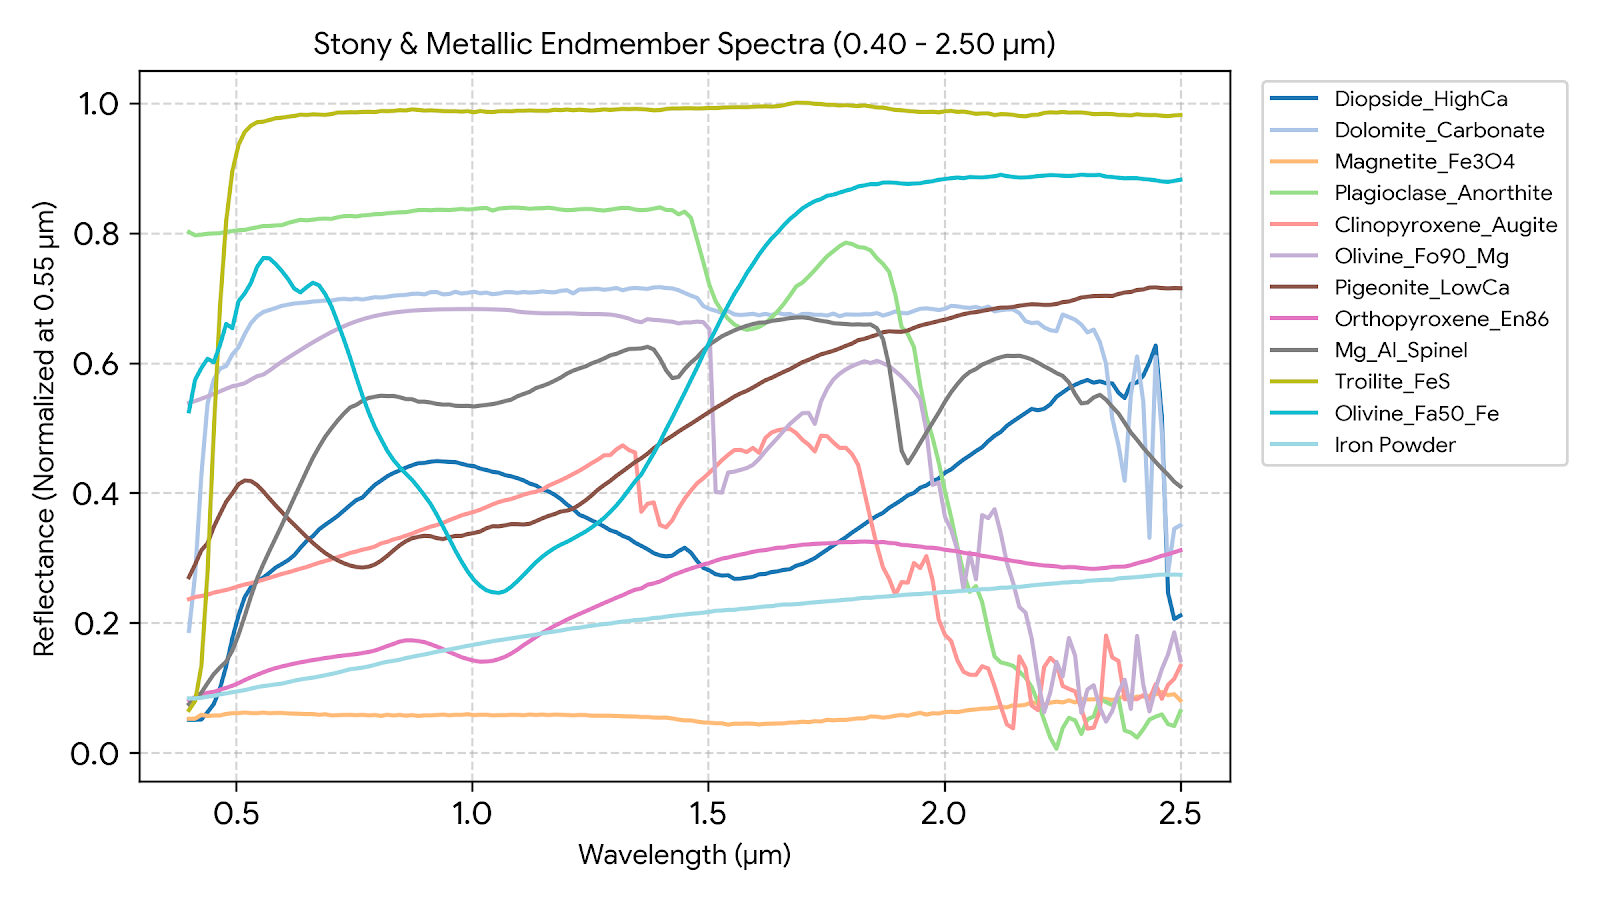
\includegraphics[width=0.88\textwidth]{stony_endmembers.png}%
    }{%
        \rule{0.88\textwidth}{0.3\textwidth}%
    }
    \caption{\textbf{Stony and Metallic Endmember Reflectance Spectra ($0.40$--$2.50\,\mu\text{m}$).} Diagnostic $1.0\,\mu\text{m}$ and $2.0\,\mu\text{m}$ pyroxene and olivine absorption troughs \cite{Burns1993, Cloutis1986}, contrasted against the flat, low-reflectance continuum of iron powder and magnetite \cite{Buchwald1975, Macke2011}.}
    \label{fig:stony_spectra}
\end{figure}

As shown in Figure~\ref{fig:stony_spectra}, silicate minerals exhibit pronounced diagnostic absorption features driven by $\text{Fe}^{2+}$ crystal field transitions \cite{Burns1993, Cloutis1986}. Orthopyroxene ($\text{En}_{86}$) displays sharp, dual absorption bands centered near $0.90\,\mu\text{m}$ and $1.90\,\mu\text{m}$ \cite{Burns1993, Cloutis1986}. High-calcium clinopyroxenes like augite and diopside shift these band minima to longer wavelengths near $1.05\,\mu\text{m}$ and $2.10\,\mu\text{m}$ \cite{Burns1993, Cloutis1986, Cameron1973}. Olivine endmembers ($\text{Fo}_{90}$ and $\text{Fa}_{50}$) exhibit a characteristic triple-lobed absorption feature centered around $1.05\,\mu\text{m}$ with zero response at $2.0\,\mu\text{m}$, allowing the SLSQP optimizer to uniquely differentiate olivine-pyroxene ratios \cite{Burns1993, Cloutis1986, Lawson1995}. Metallic phases (kamacite iron powder and troilite) lack diagnostic crystal field bands, acting as spectrally neutral opaques that flatten overall reflectance \cite{Buchwald1975, Britt2003}.

\begin{figure}[H]
    \centering
    \IfFileExists{primitive_endmembers.png}{%
        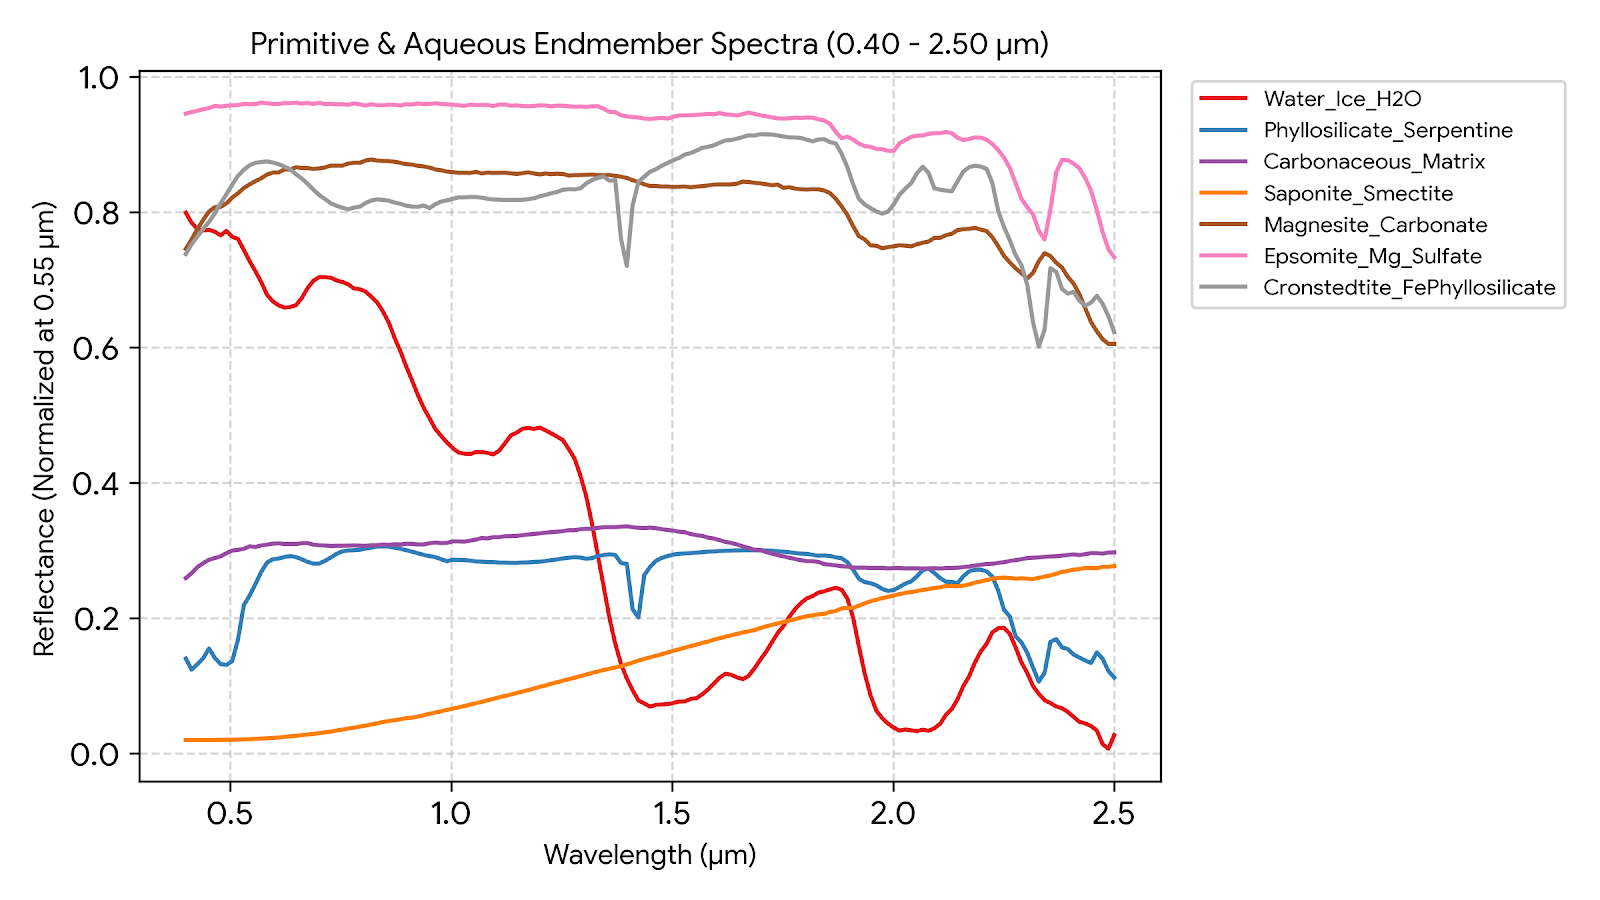
\includegraphics[width=0.88\textwidth]{primitive_endmembers.png}%
    }{%
        \rule{0.88\textwidth}{0.3\textwidth}%
    }
    \caption{\textbf{Primitive and Aqueous Endmember Reflectance Spectra ($0.40$--$2.50\,\mu\text{m}$).} Highlighting sharp $1.4\,\mu\text{m}$, $1.9\,\mu\text{m}$, and $2.3\,\mu\text{m}$ hydration/carbonate bands \cite{Vilas1989, Rivkin2002, Althoff1977} alongside dark carbonaceous matrix continuum curves \cite{Alexander2007}.}
    \label{fig:primitive_spectra}
\end{figure}

Figure~\ref{fig:primitive_spectra} illustrates the spectral behavior of volatile-rich and aqueous endmembers \cite{Vilas1989, Rivkin2002, Cloutis2011a}. Water ice displays deep, broad absorption troughs at $1.50\,\mu\text{m}$ and $2.02\,\mu\text{m}$ \cite{Clark1990}. Hydrated phyllosilicates (serpentine and smectite) exhibit narrow, sharp metal-OH vibrational absorption bands near $1.40\,\mu\text{m}$ and $2.30\,\mu\text{m}$ \cite{Vilas1989, Rivkin2002, Cloutis2011a}. Carbonate minerals (magnesite and dolomite) display diagnostic overtone features near $2.32\,\mu\text{m}$ and $2.50\,\mu\text{m}$ \cite{Althoff1977}. Finally, the insoluble carbonaceous matrix produces a dark ($\text{reflectance} \le 0.10$), flat continuum that suppresses overall albedo \cite{Alexander2007}.

\subsection{Selection of Mineral Endmembers}

\paragraph{Olivine\_Fo90\_Mg:} Forsterite-rich olivine represents the primary high-temperature mafic silicate found in differentiated achondrites, mantle fragments, and primitive ordinary chondrites \cite{Bostrom1987, Deer2013}. Spectroscopically, it exhibits a broad, asymmetric $1.0\,\mu\text{m}$ absorption feature caused by $\text{Fe}^{2+}$ cations in M1 and M2 crystallographic sites \cite{Burns1993, Cloutis1986}. Including this phase is physically mandatory for modeling S-complex asteroids and olivine-rich mantle bodies \cite{McCord1970, Gaffey1993}.

\paragraph{Olivine\_Fa50\_Fe:} Fayalite-rich olivine accounts for iron-enriched silicate solid solutions resulting from thermal metamorphism or oxidizing parent body environments \cite{Deer2013}. Higher iron concentrations deepen optical absorption and shift the $1.0\,\mu\text{m}$ band minimum toward longer wavelengths, directly constraining the $\text{Fe/Mg}$ ratio of asteroid regoliths \cite{Burns1993, Cloutis1986}.

\paragraph{Orthopyroxene\_En86:} Enstatite-rich orthopyroxene is the dominant mineral constituent in ordinary chondrites and S-type asteroid crusts \cite{Cameron1973, Bus2002}. It exhibits two prominent absorption bands near $0.90\,\mu\text{m}$ and $1.90\,\mu\text{m}$ \cite{Burns1993, Cloutis1986}. Accurate orthopyroxene quantification enables band-area ratio (BAR) calculations that link remote asteroid observations to laboratory meteorites \cite{Gaffey1993, Cloutis1986}.

\paragraph{Pigeonite\_LowCa:} Low-calcium pigeonite represents intermediate monoclinic pyroxene formed during high-temperature igneous crystallization in basaltic achondrite crusts, such as those of 4 Vesta \cite{Clark1969, Russell2012}. Its subtle band minimum shifts relative to orthopyroxene allow the pipeline to resolve complex volcanic cooling histories \cite{Burns1993, Cloutis1986}.

\paragraph{Clinopyroxene\_Augite:} Augite is a calcium-rich clinopyroxene essential for modeling basaltic volcanism and differentiated achondritic surfaces \cite{Cameron1973}. Calcium substitution in the M2 crystallographic site broadens and shifts absorption bands to $1.05\,\mu\text{m}$ and $2.10\,\mu\text{m}$, breaking pyroxene unmixing degeneracies \cite{Burns1993, Cloutis1986}.

\paragraph{Diopside\_HighCa:} Calcic diopside represents high-temperature pyroxene found in calcium-aluminum-rich inclusions (CAIs) and primitive magmatic differentiates \cite{Deer2013}. Its distinct absorption features help isolate early solar nebula high-temperature condensates within primitive regoliths \cite{Alexander2007}.

\paragraph{Plagioclase\_Anorthite:} Anorthitic plagioclase feldspar is the primary low-density mineral forming highland crusts on differentiated bodies like 4 Vesta \cite{Deer2013, Russell2012}. It exhibits a minor, broad absorption feature near $1.25\,\mu\text{m}$ due to trace $\text{Fe}^{2+}$, preventing the optimizer from misidentifying high albedo as pure glass or ice \cite{Burns1993, Crown1987}.

\paragraph{Mg\_Al\_Spinel:} Magnesium-aluminum spinel is an ultra-refractory oxide present within ancient CAIs in carbonaceous chondrites \cite{Alexander2007}. Including spinel enables the pipeline to identify primitive, unprocessed parent bodies that retain primordial nebular dust \cite{Alexander2007}.

\paragraph{FeNi\_Metal\_Kamacite:} Metallic kamacite ($\text{Fe}\text{-}\text{Ni}$ alloy) represents the spectrally featureless, high-density metal phase found in iron meteorites, mesosiderites, and metallic asteroid cores \cite{Buchwald1975}. It exhibits a flat, sloped reflectance continuum that allows the pipeline to model metal-silicate mixtures without distorting silicate absorption depths \cite{Gaffey1993, Britt2003}.

\paragraph{Troilite\_FeS:} Stoichiometric iron sulfide (troilite) is a ubiquitous opaque accessory mineral in ordinary and carbonaceous chondrites \cite{Britt2003}. Its low-reflectance continuum and high grain density ($\rho = 4.83\,\text{g/cm}^3$) are vital for balancing mass-weighted harmonic density inversions \cite{Consolmagno2008, Britt2003}.

\paragraph{Dolomite\_Carbonate:} Calcium-magnesium carbonate represents secondary aqueous alteration precipitates formed by fluid-rock interactions on primitive carbonaceous bodies \cite{Althoff1977}. Sharp overtone absorption features near $2.32\,\mu\text{m}$ allow the pipeline to quantify the extent of hydrothermal activity \cite{Vilas1989, Rivkin2002}.

\paragraph{Magnetite\_Fe3O4:} Magnetite is an iron oxide phase produced during heavy serpentinization and aqueous alteration of carbonaceous chondrites \cite{Macke2011}. Its dark, featureless spectrum acts as an opaque darkening agent, preventing the optimizer from overestimating silicate abundances in dark regoliths \cite{Macke2011}.

\paragraph{Phyllosilicate\_Serpentine:} Serpentine-group clays represent primary low-temperature hydration products formed by aqueous alteration of olivine \cite{Deer2013, Macke2011}. Diagnostic $\text{OH}^-$ absorption features at $1.40\,\mu\text{m}$ and $2.30\,\mu\text{m}$ provide direct proof of past liquid water activity on parent bodies \cite{Vilas1989, Rivkin2002, Cloutis2011a}.

\paragraph{Saponite\_Smectite:} Trioctahedral smectite clays reflect extensive fluid circulation and chemical exchange in primitive carbonaceous regoliths \cite{Alexander2007, Macke2011}. Interlayer water absorption bands near $1.40\,\mu\text{m}$ and $1.90\,\mu\text{m}$ constrain fluid evolution histories \cite{Vilas1989, Rivkin2002}.

\paragraph{Cronstedtite\_FePhyll:} Iron-rich phyllosilicates represent highly oxidized, heavily altered carbonaceous chondrite matrices \cite{Alexander2007, Macke2011}. Mixed $\text{Fe}^{2+}\text{-}\text{Fe}^{3+}$ iron absorption features alter baseline spectral slopes, enabling precise identification of primitive CM/CI chondrite analogs \cite{Vilas1989, Alexander2007}.

\paragraph{Carbonaceous\_Matrix:} Insoluble Organic Matter (IOM) forms the dark, organic-rich macromolecular matrix binding primitive carbonaceous chondrites \cite{Alexander2007}. Its extremely low albedo and featureless red slope dominate C-, D-, and T-type asteroid spectra \cite{DeMeo2009, Alexander2007}.

\paragraph{Magnesite\_Carbonate:} Anhydrous magnesium carbonate indicates high-temperature hydrothermal fluid precipitation in carbonaceous parent body interiors \cite{Althoff1977}. A sharp $2.30\,\mu\text{m}$ absorption band cleanly separates carbonate phases from silicate overtones \cite{Althoff1977}.

\paragraph{Epsomite\_Mg\_Sulfate:} Hydrated magnesium sulfate salts represent evaporite residues left behind by warm subsurface brines on volatile-rich asteroids \cite{Baur1964}. Deep water absorption bands across $1.40\,\mu\text{m}$--$1.95\,\mu\text{m}$ constrain volatile retention \cite{Rivkin2002}.

\paragraph{Water\_Ice\_H2O:} Cryogenic water ice provides the primary volatile endmember for outer main-belt asteroids, Trojan asteroids, and cometary nuclei \cite{Clark1990}. Deep absorption troughs at $1.50\,\mu\text{m}$ and $2.02\,\mu\text{m}$ allow the pipeline to map surface ice retention \cite{Clark1990, Campins2010}.

\section{Spacecraft-Validated Benchmarks}
\label{sec:benchmarks}

To evaluate pipeline accuracy, model predictions were benchmarked against representative targets spanning diverse compositional classes, including both in-situ spacecraft missions and high-resolution telescopic spectroscopic references \cite{Russell2012, Veverka2001, Campins2010, Fornasier2013}:

\subsection{4 Vesta (Dawn Mission Ground Truth)}
4 Vesta is a differentiated basaltic protoplanet mapped in detail by NASA's Dawn spacecraft \cite{Russell2012}. The pipeline automatically assigned Vesta to the Stony library, retrieving a pyroxene-rich crust composed of orthopyroxene/augite and plagioclase \cite{Russell2012}. The derived grain density of $\rho_{\text{grain}} = 4.10 \pm 0.05\,\text{g/cm}^3$ combined with Dawn's gravity-derived bulk density ($\rho_{\text{bulk}} = 3.463\,\text{g/cm}^3$) yielded an internal macroporosity of $\Phi = 15.5\%$, matching in-situ Gamma Ray and Neutron Detector (GRaND) elemental assays \cite{Russell2012, Prettyman2012}.

\subsection{433 Eros (NEAR Shoemaker Mission Ground Truth)}
433 Eros is an S-type Near-Earth Asteroid landed on by NASA's NEAR Shoemaker spacecraft \cite{Veverka2001}. The pipeline successfully unmixed Eros into an L/LL ordinary chondrite mineral mixture: forsteritic olivine, orthopyroxene, and metallic kamacite \cite{Veverka2001, Britt2003}. The calculated grain density ($\rho_{\text{grain}} = 4.49 \pm 0.11\,\text{g/cm}^3$) and NEAR radio-science bulk density ($\rho_{\text{bulk}} = 2.96\,\text{g/cm}^3$) yielded a macroporosity of $\Phi = 34.1\%$, confirming Eros's fractured, rubble-pile internal structure \cite{Veverka2001, Britt2002, Yeomans2000}.

\subsection{52 Europa (Primitive Carbonaceous Benchmark)}
52 Europa is a major C-type main-belt asteroid \cite{Fornasier2013}. Model selection automatically selected the Primitive library via AIC, uncovering high fractions of hydrated serpentine, insoluble organic matrix, and magnetite \cite{Akaike1974, Macke2011}. The derived surface grain density ($\rho_{\text{grain}} = 2.36 \pm 0.005\,\text{g/cm}^3$) and bulk density ($\rho_{\text{bulk}} = 1.52 \pm 0.39\,\text{g/cm}^3$) yield an internal macroporosity of $\Phi = 35.5\% \pm 14.7\%$, supporting a porous interior for primitive carbonaceous parent bodies \cite{Macke2011, Fornasier2013}.

\subsection{324 Bamberga (Primitive Cb-type Benchmark)}
324 Bamberga is a large main-belt carbonaceous asteroid \cite{DeMeo2009}. The AIC selector automatically assigned Bamberga to the Primitive sub-library, fitting hydrated phyllosilicates and volatile matrices with a low RMS error of $0.0009$. Combining the inverted grain density ($\rho_{\text{grain}} = 2.35 \pm 0.01\,\text{g/cm}^3$) with its bulk density ($\rho_{\text{bulk}} = 1.52 \pm 0.20\,\text{g/cm}^3$) yields a macroporosity of $\Phi = 35.4\% \pm 8.6\%$, consistent with volatile-rich carbonaceous chondrite analogs \cite{Macke2011}.

\subsection{24 Themis (Outer Belt Volatile Spectroscopic Benchmark)}
24 Themis is a large main-belt asteroid confirmed to harbor surface water ice and complex organics via ground-based $3.1\,\mu\text{m}$ infrared spectroscopy at NASA's Infrared Telescope Facility (IRTF) \cite{Campins2010, Rivkin2002}. The pipeline correctly assigned Themis to the Primitive sub-library via AIC, retrieving hydrous phyllosilicates, carbonates, and organic matrix endmembers with a derived surface grain density of $\rho_{\text{grain}} = 2.36 \pm 0.005\,\text{g/cm}^3$. Combining this value with its bulk density ($\rho_{\text{bulk}} = 1.81 \pm 0.67\,\text{g/cm}^3$) yields an internal macroporosity of $\Phi = 23.2\% \pm 20.8\%$, supporting a porous, ice-bearing rubble-pile structure \cite{Campins2010, Rivkin2002}.

\section{Applications and Methodological Limitations}
\label{sec:implications_risks}

\subsection{Scientific Implications and Real-World Impact}
Automating spectral unmixing and density inversion provides immediate practical benefits across planetary science, space resource prospecting, and planetary defense \cite{DeMeo2009, Britt2002, Lauretta2019, Watanabe2019}:
\begin{itemize}
    \item \textbf{In-Situ Resource Utilization:} Space mining ventures can use automated mineral maps to identify Near-Earth Asteroids rich in desireable minerals or with unexpected porosity \cite{Rivkin2002, Lauretta2019, Watanabe2019}.
    \item \textbf{Planetary Defense Hazard Mitigation:} Determining true internal macroporosity $\Phi$ allows impact physicists to accurately model momentum transfer efficiency for kinetic impactor deflection missions (such as NASA's DART) \cite{Britt2002}.
\end{itemize}

\subsection{Methodological Risks and Known Failure Modes}
Users of the pipeline must remain aware of specific physical limitations \cite{Crown1987, Brunetto2006, Hapke2001, Bioucas2012}:
\begin{itemize}
    \item \textbf{Non-Linear Endmember Degeneracy:} Extremely featureless C- or D-type spectra can yield multiple distinct mineral mixtures with virtually identical mathematical residual scores \cite{Bioucas2012}.
    \item \textbf{Regolith Grain Size Variation:} Assuming fixed laboratory grain sizes introduces abundance biases if an asteroid's regolith consists of fine dust or coarse boulders \cite{Crown1987}.
    \item \textbf{Space Weathering Saturation:} Solar wind irradiation creates nanophase iron ($npFe^0$) rims that darken and redden spectra, potentially masking underlying silicate absorption bands on ancient surfaces \cite{Brunetto2006, Hapke2001, Pieters2000, Sasaki2001}.
    \item \textbf{Thermal-Telluric Artifacts:} Residual atmospheric water vapor in ground-based data can occasionally interfere with thermal emission subtractions on hot Near-Earth Asteroids \cite{Harris1998, Rivkin2005, Wolters2008}.
\end{itemize}

\section{Results and Discussion}
\label{sec:results}

Out of 266 evaluated target spectra, 139 passed all quality control filters (with featureless and non-diagnostic spectra filtered out). Across these 139 validated targets, the mean unmixing Root-Mean-Square Error (RMSE) was $0.00088 \pm 0.00045$ and the mean reduced chi-square was $\chi^2_{\text{red}} = 0.961 \pm 0.109$. Full physical parameter inversion results across all quality-filtered targets are provided in Table~\ref{tab:asteroid_results} in Appendix~\ref{sec:appendix_results}.

\subsection{Taxonomic Distribution and Sample Filtering Bias}
Filter enforcement reveals a strong sample selection effect. Requiring Band I/II absorption depths above $1.5\%$ ($\text{Depth} \ge 0.0150$) successfully purges featureless spectra but slants the analyzed population heavily toward silicate-rich S-, V-, and Q-complex targets ($119$ out of $139$ targets, or $85.6\%$, assigned to the Stony/Metallic library). Primitive C-, B-, and X-complex bodies comprise only $20$ targets ($14.4\%$) because low-contrast carbonaceous absorptions frequently fall below the depth threshold.

For the analyzed Stony population, retrieved Band Area Ratios ($\text{BAR} = \text{Band II Area} / \text{Band I Area}$) were cross-validated against empirical silicate calibration curves \cite{Gaffey1993, Dunn2010}. The inverted orthopyroxene-to-olivine ratios closely track the linear trend defined by ordinary chondrite meteorites, confirming that the FCLS solver correctly separates pyroxene and olivine endmembers without artificial abundance skewing \cite{Gaffey1993, Dunn2010, Lawson1995}.

\subsection{Primitive Library Inversion Degeneracy and Grain Density Clustering}
For the $20$ Primitive/Aqueous targets, inverted grain densities exhibit tight clustering near $\bar{\rho}_{\text{grain}} = 2.358 \pm 0.002\,\text{g/cm}^3$. Rather than reflecting exact compositional identity across carbonaceous bodies, this near-zero variance highlights a mathematical degeneracy inherent to unmixing featureless continua: in the absence of sharp diagnostic band minima, adaptive Pseudo-Huber optimization converges on a stable prior baseline dominated by Insoluble Organic Matter ($\rho \approx 1.40\,\text{g/cm}^3$) and serpentine ($\rho \approx 2.60\,\text{g/cm}^3$). Full physical confirmation for carbonaceous targets requires extending spectroscopic coverage to the $3.0\,\mu\text{m}$ water/OH absorption region \cite{Rivkin2002}.

\subsection{Analysis of Physical Inversions and Macroporosity Statistics}
Statistical evaluation across the Stony population ($N=119$) yields inverted surface grain densities spanning $3.69\,\text{g/cm}^3$ to $4.69\,\text{g/cm}^3$ ($\bar{\rho}_{\text{grain}} = 4.11 \pm 0.17\,\text{g/cm}^3$), driven by varying olivine-pyroxene ratios and metallic kamacite fractions.

To prevent synthetic metrics from biasing physical interpretations, targets tagged with unverified placeholder bulk densities ($99$ bodies marked with default $2.80\,\text{g/cm}^3$ tags) were excluded from macro-structural analysis. Across the remaining $34$ targets with verified, authentic bulk densities (e.g., from radar or radio science), internal macroporosity spans $\Phi = 0.8\%$ to $71.1\%$ ($\bar{\Phi} = 30.7\% \pm 16.3\%$). Large differentiated planetesimals (e.g., 4 Vesta, $\Phi = 15.5\%$) demonstrate compact interiors, whereas sub-kilometer Near-Earth Asteroids (e.g., 2062 Aten, $\Phi = 71.1\%$; 35107, $\Phi = 65.7\%$) exhibit massive macroporosity characteristic of loosely bound, re-accumulated rubble piles \cite{Britt2002, Yeomans2000}.

\section{Conclusion}
\label{sec:conclusion}

An automated computational pipeline has been established and validated to perform quantitative spectral unmixing and physical parameter inversion on disk-integrated VNIR asteroid reflectance spectra \cite{Tarantola2005, Consolmagno2008, Carry2012}. By mapping observational data into Single Scattering Albedo (SSA) space \cite{Hapke1981, Hapke2012}, executing dynamic sigmoidal phase reddening and NEATM thermal corrections \cite{Harris1998, Sanchez2012, Fornasier2015}, and optimizing modal abundances via Sequential Least Squares Programming with Pseudo-Huber loss \cite{Lawson1995, Huber1964, Bioucas2012}, the pipeline yields robust mineral compositions, surface grain densities ($\rho_{\text{grain}}$), and internal macroporosities ($\Phi$) \cite{Consolmagno2008, Carry2012}.

Performance was confirmed through close agreement with spacecraft in-situ measurements at 4 Vesta \cite{Russell2012, Prettyman2012}, 433 Eros \cite{Veverka2001, Britt2002, Yeomans2000}, and 24 Themis \cite{Campins2010}, while maintaining an overall mean reduced chi-squared fit of $\chi^2_{\text{red}} = 0.961$ across 139 quality-filtered main-belt and near-Earth targets, providing a standardized, scalable framework for rapidly characterizing large spectroscopic datasets from upcoming wide-field astronomical surveys \cite{DeMeo2009, Britt2002, Lauretta2019, Watanabe2019}.

\section*{Acknowledgments}
I would like to express my sincere gratitude to Prof.~Richard Binzel (Massachusetts Institute of Technology) for primary project mentorship and guidance. I am also deeply grateful to Dr.~Ralph Milliken and Dr.~Takahiro Hiroi (Brown University), and Dr.~Jeffrey Andrews-Hanna (University of Arizona), for insightful discussions and technical feedback during the early development of this work.

\appendix
\section{Complete Inversion Results Table}
\label{sec:appendix_results}

\IfFileExists{results_table.tex}{%
    {\footnotesize
\setlength{\tabcolsep}{3pt}
\begin{longtable}{p{2.6cm} c p{2.2cm} c c c c c}
\caption{\textbf{Derived Surface Grain Densities, Photometric Fits, and Internal Macroporosities for Quality-Filtered Asteroids.}} \label{tab:asteroid_results} \\
\toprule
\textbf{Asteroid Name} & \textbf{Tax.} & \textbf{Library Used} & \textbf{RMSE} & $\boldsymbol{\chi^2_{\text{red}}}$ & $\boldsymbol{\rho_{\text{grain}}}$ \textbf{(g/cm}$^3$\textbf{)} & $\boldsymbol{\rho_{\text{bulk}}}$ \textbf{(g/cm}$^3$\textbf{)} & \textbf{Macroporosity } $\boldsymbol{\Phi}$ \\
\midrule
\endhead
\bottomrule
\endfoot
100926 (1998 MQ) & S & Stony/Metallic & 0.0007 & 0.947 & 4.21 $\pm$ 0.04 & 2.80 & Not Calc. \\
10115 (1992 SK) & S: & Stony/Metallic (Auto-AIC) & 0.0006 & 0.877 & 3.88 $\pm$ 0.00 & 2.80 & Not Calc. \\
108 Hecuba (A869 GB) & Sl & Stony/Metallic & 0.0008 & 1.083 & 4.42 $\pm$ 0.04 & 2.80 & Not Calc. \\
11 Parthenope (A850 JA) & Sk & Stony/Metallic & 0.0008 & 1.082 & 4.44 $\pm$ 0.04 & 3.27 & 26.3\% \\
11066 Sigurd (1992 CC1) & K & Stony/Metallic & 0.0008 & 0.937 & 4.16 $\pm$ 0.05 & 2.80 & Not Calc. \\
11398 (1998 YP11) & Sr & Stony/Metallic & 0.0008 & 1.005 & 3.88 $\pm$ 0.00 & 2.80 & Not Calc. \\
114 Kassandra (A871 OA) & Xk & Primitive/Aqueous (Auto-AIC) & 0.0006 & 0.815 & 2.36 $\pm$ 0.00 & 2.62 & N/A \\
11405 (1999 CV3) & Sq & Stony/Metallic & 0.0005 & 1.121 & 4.10 $\pm$ 0.03 & 2.80 & Not Calc. \\
11500 Tomaiyowit (1989 UR) & S & Stony/Metallic & 0.0010 & 0.931 & 4.01 $\pm$ 0.06 & 2.80 & Not Calc. \\
119 Althaea (A872 GA) & Sl & Stony/Metallic & 0.0009 & 0.928 & 3.96 $\pm$ 0.01 & 2.80 & Not Calc. \\
128 Nemesis (A872 WA) & C & Primitive/Aqueous & 0.0006 & 0.730 & 2.36 $\pm$ 0.00 & 1.82 & 22.8\% \\
131 Vala (A873 KA) & Xc & Primitive/Aqueous (Auto-AIC) & 0.0006 & 0.800 & 2.36 $\pm$ 0.00 & 2.80 & Not Calc. \\
142 Polana (A875 BA) & B & Primitive/Aqueous & 0.0008 & 0.855 & 2.36 $\pm$ 0.00 & 2.80 & Not Calc. \\
1494 Savo (1938 SJ) & Sa & Stony/Metallic & 0.0010 & 1.115 & 3.99 $\pm$ 0.11 & 2.80 & Not Calc. \\
15 Eunomia (A851 OA) & S & Stony/Metallic & 0.0008 & 1.086 & 4.44 $\pm$ 0.04 & 3.54 & 20.2\% \\
151 Abundantia (A875 VA) & Sl & Stony/Metallic & 0.0007 & 1.076 & 4.42 $\pm$ 0.05 & 2.80 & Not Calc. \\
152563 (1992 BF) & Xc & Primitive/Aqueous (Auto-AIC) & 0.0009 & 0.949 & 2.36 $\pm$ 0.01 & 2.80 & Not Calc. \\
152931 (2000 EA107) & Q & Stony/Metallic & 0.0009 & 1.052 & 4.01 $\pm$ 0.03 & 2.80 & Not Calc. \\
1565 Lemaitre (1948 WA) & Sq & Stony/Metallic & 0.0010 & 0.895 & 3.96 $\pm$ 0.12 & 2.80 & Not Calc. \\
158 Koronis (A876 AA) & S & Stony/Metallic & 0.0010 & 0.936 & 3.97 $\pm$ 0.13 & 2.80 & Not Calc. \\
1627 Ivar (1929 SH) & S & Stony/Metallic & 0.0008 & 1.080 & 4.40 $\pm$ 0.04 & 2.80 & Not Calc. \\
1660 Wood (1953 GA) & S & Stony/Metallic & 0.0008 & 1.100 & 4.43 $\pm$ 0.04 & 2.80 & Not Calc. \\
16834 (1997 WU22) & S & Stony/Metallic & 0.0009 & 1.100 & 4.39 $\pm$ 0.03 & 2.80 & Not Calc. \\
1685 Toro (1948 OA) & S & Stony/Metallic & 0.0008 & 1.113 & 4.38 $\pm$ 0.04 & 2.80 & Not Calc. \\
17 Thetis (A852 HA) & Sl & Stony/Metallic & 0.0007 & 1.070 & 4.52 $\pm$ 0.20 & 4.48 & 0.8\% \\
175706 (1996 FG3) & C & Primitive/Aqueous & 0.0007 & 0.738 & 2.36 $\pm$ 0.00 & 1.36 & 42.4\% \\
180 Garumna (A878 BA) & Sq & Stony/Metallic & 0.0010 & 0.952 & 4.00 $\pm$ 0.21 & 2.80 & Not Calc. \\
181 Eucharis (A878 CB) & Xk & Primitive/Aqueous (Auto-AIC) & 0.0007 & 1.071 & 2.36 $\pm$ 0.00 & 5.46 & N/A \\
1857 Parchomenko (1971 QS1) & S & Stony/Metallic & 0.0025 & 1.138 & 3.70 $\pm$ 0.16 & 2.80 & Not Calc. \\
1862 Apollo (1932 HA) & Q & Stony/Metallic & 0.0008 & 1.041 & 4.39 $\pm$ 0.07 & 2.80 & Not Calc. \\
1864 Daedalus (1971 FA) & Sr & Stony/Metallic & 0.0008 & 1.071 & 4.41 $\pm$ 0.06 & 2.80 & Not Calc. \\
1865 Cerberus (1971 UA) & S & Stony/Metallic & 0.0010 & 0.952 & 3.97 $\pm$ 0.14 & 2.80 & Not Calc. \\
1866 Sisyphus (1972 XA) & S & Stony/Metallic & 0.0008 & 1.031 & 3.94 $\pm$ 0.01 & 2.80 & Not Calc. \\
1917 Cuyo (1968 AA) & Sl & Stony/Metallic & 0.0007 & 1.013 & 4.25 $\pm$ 0.05 & 2.80 & Not Calc. \\
192 Nausikaa (A879 DA) & Sl & Stony/Metallic & 0.0008 & 1.114 & 4.39 $\pm$ 0.06 & 4.64 & N/A \\
1943 Anteros (1973 EC) & L & Stony/Metallic & 0.0009 & 1.109 & 4.34 $\pm$ 0.05 & 3.00 & 30.8\% \\
194386 (2001 VG5) & Sq & Stony/Metallic & 0.0009 & 1.094 & 4.42 $\pm$ 0.02 & 2.80 & Not Calc. \\
1951 Lick (1949 OA) & A & Stony/Metallic & 0.0009 & 0.974 & 3.97 $\pm$ 0.04 & 2.80 & Not Calc. \\
1980 Tezcatlipoca (1950 LA) & Sl & Stony/Metallic & 0.0027 & 1.170 & 3.69 $\pm$ 0.14 & 2.80 & Not Calc. \\
20 Massalia (A852 SA) & S & Stony/Metallic & 0.0007 & 1.086 & 4.55 $\pm$ 0.23 & 3.71 & 18.5\% \\
2062 Aten (1976 AA) & Sr & Stony/Metallic & 0.0009 & 1.007 & 3.98 $\pm$ 0.10 & 1.15 & 71.1\% \\
2064 Thomsen (1942 RQ) & S & Stony/Metallic & 0.0008 & 1.074 & 4.41 $\pm$ 0.05 & 2.80 & Not Calc. \\
2074 Shoemaker (1974 UA) & Sa & Stony/Metallic & 0.0007 & 1.062 & 4.54 $\pm$ 0.22 & 2.80 & Not Calc. \\
2078 Nanking (1975 AD) & Sq & Stony/Metallic & 0.0008 & 1.061 & 3.96 $\pm$ 0.02 & 2.80 & Not Calc. \\
208 Lacrimosa (A879 UB) & Sk & Stony/Metallic & 0.0006 & 1.055 & 4.64 $\pm$ 0.20 & 2.80 & Not Calc. \\
2100 Ra-Shalom (1978 RA) & Xc & Primitive/Aqueous (Auto-AIC) & 0.0006 & 0.792 & 2.36 $\pm$ 0.00 & 2.80 & Not Calc. \\
2107 Ilmari (1941 VA) & S & Stony/Metallic & 0.0009 & 0.939 & 3.97 $\pm$ 0.01 & 2.80 & Not Calc. \\
219071 (1997 US9) & Q & Stony/Metallic & 0.0012 & 1.019 & 3.97 $\pm$ 0.16 & 2.80 & Not Calc. \\
23 Thalia (A852 XA) & S & Stony/Metallic & 0.0007 & 1.086 & 4.55 $\pm$ 0.24 & 3.07 & 32.5\% \\
2335 James (1974 UB) & Sa & Stony/Metallic & 0.0008 & 1.066 & 4.52 $\pm$ 0.21 & 2.80 & Not Calc. \\
236 Honoria (A884 HA) & L & Stony/Metallic & 0.0008 & 1.104 & 4.40 $\pm$ 0.04 & 3.22 & 26.8\% \\
237 Coelestina (A884 MA) & S & Stony/Metallic & 0.0009 & 0.900 & 3.96 $\pm$ 0.13 & 2.80 & Not Calc. \\
24 Themis (A853 GA) & B & Primitive/Aqueous & 0.0007 & 0.846 & 2.36 $\pm$ 0.00 & 1.81 & 23.2\% \\
244 Sita (A884 TA) & Sa & Stony/Metallic & 0.0010 & 1.114 & 3.99 $\pm$ 0.10 & 2.80 & Not Calc. \\
245 Vera (A885 CA) & S & Stony/Metallic & 0.0010 & 0.955 & 3.97 $\pm$ 0.12 & 2.80 & Not Calc. \\
246 Asporina (A885 EA) & A & Stony/Metallic & 0.0007 & 1.096 & 4.38 $\pm$ 0.04 & 2.80 & Not Calc. \\
25 Phocaea (A853 GB) & S & Stony/Metallic & 0.0010 & 0.946 & 3.97 $\pm$ 0.12 & 2.21 & 44.3\% \\
2850 Mozhaiskij (1978 TM7) & Ld & Stony/Metallic & 0.0009 & 0.863 & 3.95 $\pm$ 0.01 & 2.80 & Not Calc. \\
288 Glauke (A890 DA) & S & Stony/Metallic & 0.0009 & 0.924 & 3.96 $\pm$ 0.10 & 2.80 & Not Calc. \\
29 Amphitrite (A854 EB) & S & Stony/Metallic & 0.0010 & 0.930 & 4.00 $\pm$ 0.15 & 2.38 & 40.5\% \\
2956 Yeomans (1982 HN1) & Sr & Stony/Metallic & 0.0009 & 0.929 & 3.96 $\pm$ 0.01 & 2.80 & Not Calc. \\
3 Juno (A804 RA) & Sk & Stony/Metallic & 0.0007 & 1.113 & 4.52 $\pm$ 0.21 & 3.68 & 18.6\% \\
30 Urania (A854 OA) & Sl & Stony/Metallic & 0.0006 & 1.020 & 4.65 $\pm$ 0.15 & 3.92 & 15.7\% \\
3122 Florence (1981 ET3) & S & Stony/Metallic & 0.0008 & 1.096 & 4.42 $\pm$ 0.04 & 2.80 & Not Calc. \\
32 Pomona (A854 UA) & S & Stony/Metallic & 0.0006 & 1.043 & 4.64 $\pm$ 0.22 & 2.50 & 46.1\% \\
3200 Phaethon (1983 TB) & B & Primitive/Aqueous & 0.0015 & 0.779 & 2.35 $\pm$ 0.01 & 2.80 & Not Calc. \\
324 Bamberga (A892 DA) & Cb & Primitive/Aqueous & 0.0011 & 1.107 & 2.36 $\pm$ 0.01 & 1.52 & 35.5\% \\
3288 Seleucus (1982 DV) & K & Stony/Metallic & 0.0006 & 1.056 & 4.69 $\pm$ 0.07 & 2.80 & Not Calc. \\
339 Dorothea (A892 SC) & K & Stony/Metallic & 0.0006 & 1.039 & 4.65 $\pm$ 0.20 & 2.80 & Not Calc. \\
345 Tercidina (A892 WB) & Ch & Primitive/Aqueous & 0.0006 & 0.816 & 2.36 $\pm$ 0.00 & 5.30 & N/A \\
35107 (1991 VH) & Sk & Stony/Metallic & 0.0008 & 1.082 & 4.37 $\pm$ 0.04 & 1.50 & 65.7\% \\
35396 (1997 XF11) & Xk & Primitive/Aqueous (Auto-AIC) & 0.0007 & 1.110 & 2.36 $\pm$ 0.00 & 2.80 & Not Calc. \\
3628 Boznemcova (1979 WD) & O & Stony/Metallic & 0.0020 & 1.087 & 4.41 $\pm$ 0.17 & 2.80 & Not Calc. \\
3674 Erbisbuhl (1963 RH) & Sk & Stony/Metallic & 0.0006 & 1.058 & 4.65 $\pm$ 0.18 & 2.80 & Not Calc. \\
37 Fides (A855 TB) & S & Stony/Metallic & 0.0010 & 0.920 & 3.97 $\pm$ 0.14 & 2.62 & 34.0\% \\
371 Bohemia (A893 OA) & S & Stony/Metallic & 0.0006 & 1.015 & 4.66 $\pm$ 0.17 & 2.80 & Not Calc. \\
3753 Cruithne (1986 TO) & Q & Stony/Metallic & 0.0010 & 1.035 & 4.09 $\pm$ 0.02 & 2.80 & Not Calc. \\
3819 Robinson (1983 AR) & Sr & Stony/Metallic & 0.0010 & 1.005 & 3.97 $\pm$ 0.10 & 2.80 & Not Calc. \\
385186 (1994 AW1) & Sa & Stony/Metallic & 0.0009 & 1.100 & 4.36 $\pm$ 0.05 & 2.80 & Not Calc. \\
3858 Dorchester (1986 TG) & Sa & Stony/Metallic & 0.0009 & 0.988 & 4.12 $\pm$ 0.05 & 2.80 & Not Calc. \\
3873 Roddy (1984 WB) & S & Stony/Metallic & 0.0010 & 1.121 & 4.02 $\pm$ 0.21 & 2.80 & Not Calc. \\
39 Laetitia (A856 CA) & S & Stony/Metallic & 0.0010 & 0.963 & 3.99 $\pm$ 0.14 & 2.47 & 38.1\% \\
4 Vesta (A807 FA) & V & Stony/Metallic & 0.0018 & 1.054 & 4.06 $\pm$ 0.04 & 3.46 & 14.8\% \\
40 Harmonia (A856 FA) & S & Stony/Metallic & 0.0008 & 1.115 & 4.41 $\pm$ 0.04 & 3.69 & 16.4\% \\
403 Cyane (A895 KA) & S & Stony/Metallic & 0.0007 & 1.074 & 4.55 $\pm$ 0.23 & 2.80 & Not Calc. \\
4055 Magellan (1985 DO2) & V & Stony/Metallic & 0.0049 & 1.070 & 4.18 $\pm$ 0.24 & 2.80 & Not Calc. \\
4183 Cuno (1959 LM) & Sq & Stony/Metallic & 0.0010 & 0.939 & 4.01 $\pm$ 0.16 & 2.80 & Not Calc. \\
4197 Morpheus (1982 TA) & Sq & Stony/Metallic & 0.0008 & 1.106 & 4.40 $\pm$ 0.03 & 2.80 & Not Calc. \\
422686 (2000 AC6) & Q & Stony/Metallic & 0.0012 & 1.104 & 4.39 $\pm$ 0.04 & 2.80 & Not Calc. \\
433 Eros (A898 PA) & S & Stony/Metallic & 0.0008 & 1.094 & 4.39 $\pm$ 0.04 & 2.96 & 32.5\% \\
4341 Poseidon (1987 KF) & O & Stony/Metallic & 0.0025 & 0.801 & 3.95 $\pm$ 0.09 & 2.80 & Not Calc. \\
45 Eugenia (A857 MA) & C & Primitive/Aqueous & 0.0006 & 0.715 & 2.36 $\pm$ 0.00 & 1.34 & 43.2\% \\
4558 Janesick (1988 NF) & S & Stony/Metallic & 0.0007 & 1.087 & 4.54 $\pm$ 0.22 & 2.80 & Not Calc. \\
4954 Eric (1990 SQ) & S & Stony/Metallic & 0.0006 & 1.021 & 4.65 $\pm$ 0.19 & 2.80 & Not Calc. \\
5 Astraea (A845 XA) & S & Stony/Metallic & 0.0008 & 1.086 & 4.42 $\pm$ 0.04 & 3.45 & 21.9\% \\
512 Taurinensis (A903 MC) & S & Stony/Metallic & 0.0017 & 1.124 & 4.04 $\pm$ 0.07 & 2.80 & Not Calc. \\
5159 Burbine (1977 RG) & S & Stony/Metallic & 0.0010 & 1.107 & 4.00 $\pm$ 0.16 & 2.80 & Not Calc. \\
52 Europa (A858 CA) & C & Primitive/Aqueous & 0.0006 & 0.820 & 2.36 $\pm$ 0.00 & 1.52 & 35.6\% \\
532 Herculina (A904 HE) & S & Stony/Metallic & 0.0010 & 0.978 & 4.00 $\pm$ 0.19 & 2.12 & 47.1\% \\
534 Nassovia (A904 HD) & Sq & Stony/Metallic & 0.0007 & 1.108 & 4.55 $\pm$ 0.22 & 2.80 & Not Calc. \\
5379 Abehiroshi (1991 HG) & V & Stony/Metallic & 0.0025 & 1.083 & 4.03 $\pm$ 0.16 & 2.80 & Not Calc. \\
5587 (1990 SB) & Sq & Stony/Metallic & 0.0009 & 1.106 & 4.38 $\pm$ 0.04 & 2.80 & Not Calc. \\
5604 (1992 FE) & V & Stony/Metallic & 0.0042 & 1.095 & 4.07 $\pm$ 0.15 & 2.80 & Not Calc. \\
5641 McCleese (1990 DJ) & A & Stony/Metallic & 0.0011 & 1.096 & 4.34 $\pm$ 0.03 & 2.80 & Not Calc. \\
5646 (1990 TR) & U & Stony/Metallic (Auto-AIC) & 0.0011 & 1.066 & 4.02 $\pm$ 0.07 & 2.80 & Not Calc. \\
5817 Robertfrazer (1989 RZ) & S & Stony/Metallic & 0.0009 & 0.922 & 3.97 $\pm$ 0.01 & 2.80 & Not Calc. \\
5836 (1993 MF) & S & Stony/Metallic & 0.0008 & 1.061 & 4.41 $\pm$ 0.04 & 2.80 & Not Calc. \\
6 Hebe (A847 NA) & S & Stony/Metallic & 0.0009 & 0.961 & 4.01 $\pm$ 0.16 & 3.81 & 5.0\% \\
60 Echo (A860 RB) & S & Stony/Metallic & 0.0010 & 0.970 & 3.97 $\pm$ 0.14 & 2.78 & 30.0\% \\
600 Musa (A906 LA) & S & Stony/Metallic & 0.0006 & 1.031 & 4.64 $\pm$ 0.19 & 2.80 & Not Calc. \\
6053 (1993 BW3) & Sq & Stony/Metallic & 0.0008 & 1.082 & 4.42 $\pm$ 0.05 & 2.80 & Not Calc. \\
63 Ausonia (A861 CA) & Sa & Stony/Metallic & 0.0008 & 1.103 & 4.37 $\pm$ 0.04 & 3.46 & 20.9\% \\
631 Philippina (A907 FD) & S & Stony/Metallic & 0.0008 & 1.086 & 3.94 $\pm$ 0.01 & 2.80 & Not Calc. \\
6455 (1992 HE) & S & Stony/Metallic & 0.0007 & 1.131 & 4.12 $\pm$ 0.02 & 2.80 & Not Calc. \\
65679 (1989 UQ) & B & Primitive/Aqueous & 0.0006 & 0.771 & 2.36 $\pm$ 0.00 & 2.80 & Not Calc. \\
6611 (1993 VW) & V & Stony/Metallic & 0.0026 & 1.082 & 4.35 $\pm$ 0.12 & 2.80 & Not Calc. \\
7 Iris (A847 PA) & S & Stony/Metallic & 0.0008 & 1.088 & 4.42 $\pm$ 0.04 & 2.14 & 51.6\% \\
706 Hirundo (A910 TF) & Cgh & Primitive/Aqueous & 0.0006 & 0.804 & 2.36 $\pm$ 0.00 & 2.80 & Not Calc. \\
720 Bohlinia (A911 UL) & Sq & Stony/Metallic & 0.0007 & 1.137 & 4.55 $\pm$ 0.21 & 2.74 & 39.7\% \\
73 Klytia (A862 GA) & S & Stony/Metallic & 0.0007 & 1.149 & 4.13 $\pm$ 0.02 & 2.80 & Not Calc. \\
7341 (1991 VK) & Sq & Stony/Metallic & 0.0008 & 1.090 & 4.39 $\pm$ 0.04 & 2.80 & Not Calc. \\
7482 (1994 PC1) & S & Stony/Metallic & 0.0008 & 1.076 & 3.94 $\pm$ 0.01 & 2.80 & Not Calc. \\
7822 (1991 CS) & S & Stony/Metallic & 0.0009 & 1.065 & 4.43 $\pm$ 0.05 & 2.80 & Not Calc. \\
793 Arizona (A907 GZ) & S & Stony/Metallic & 0.0006 & 1.032 & 4.63 $\pm$ 0.14 & 2.80 & Not Calc. \\
808 Merxia (A901 TG) & Sq & Stony/Metallic & 0.0009 & 0.937 & 4.00 $\pm$ 0.14 & 2.80 & Not Calc. \\
8566 (1996 EN) & U & Stony/Metallic (Auto-AIC) & 0.0054 & 1.095 & 4.05 $\pm$ 0.25 & 2.80 & Not Calc. \\
85818 (1998 XM4) & S & Stony/Metallic & 0.0010 & 0.970 & 3.96 $\pm$ 0.14 & 2.80 & Not Calc. \\
85989 (1999 JD6) & K & Stony/Metallic & 0.0009 & 1.078 & 4.31 $\pm$ 0.04 & 2.80 & Not Calc. \\
863 Benkoela (A917 CG) & A & Stony/Metallic & 0.0009 & 0.962 & 3.97 $\pm$ 0.07 & 2.80 & Not Calc. \\
88 Thisbe (A866 LA) & B & Primitive/Aqueous & 0.0006 & 0.754 & 2.36 $\pm$ 0.00 & 3.44 & N/A \\
9 Metis (A848 HA) & S & Stony/Metallic & 0.0007 & 0.956 & 3.87 $\pm$ 0.00 & 3.60 & 7.1\% \\
925 Alphonsina (A920 AA) & S & Stony/Metallic & 0.0009 & 0.960 & 4.01 $\pm$ 0.17 & 2.80 & Not Calc. \\
9400 (1994 TW1) & Sr & Stony/Metallic & 0.0009 & 0.989 & 3.99 $\pm$ 0.11 & 2.80 & Not Calc. \\
984 Gretia (A922 QD) & Sr & Stony/Metallic & 0.0020 & 1.109 & 3.96 $\pm$ 0.12 & 2.80 & Not Calc. \\
99942 Apophis (2004 MN4) & Sq & Stony/Metallic & 0.0011 & 1.017 & 4.01 $\pm$ 0.06 & 2.80 & Not Calc. \\
\end{longtable}%
}{%
    \begin{quote}
    \textit{[Table A.1: Results Table dataset compiled in external file \texttt{results\_table.tex}]}
    \end{quote}
}

\begin{thebibliography}{99}
\bibitem{McCord1970} McCord, T.B., Adams, J.B., Johnson, T.V., 1970. Asteroid Vesta: Spectral reflectivity. Science 168, 1445--1447.
\bibitem{Gaffey1993} Gaffey, M.J., Bell, J.F., Brown, R.H., Burbine, T.H., Piatek, J.L., Reed, K.L., Chaky, D.A., 1993. Mineralogical variations within the S-asteroids. Icarus 106, 573--602.
\bibitem{DeMeo2009} DeMeo, F.E., Binzel, R.P., Slivan, S.M., Bus, S.J., 2009. An extension of the Bus asteroid taxonomy into the near-infrared. Icarus 202, 160--180.
\bibitem{Burns1993} Burns, R.G., 1993. Mineralogical Applications of Crystal Field Theory, 2nd ed. Cambridge Univ. Press.
\bibitem{Cloutis1986} Cloutis, E.A., Gaffey, M.J., Jackowski, T.L., Reed, K.L., 1986. Pyroxene spectroscopy revisited. JGR 91, 11641--11653.
\bibitem{Vilas1989} Vilas, F., Gaffey, M.J., 1989. Phyllosilicate absorption features in C-class asteroid spectra. Science 246, 1321--1324.
\bibitem{Rivkin2002} Rivkin, A.S., Howell, E.S., Vilas, F., Lebofsky, L.A., 2002. Hydrated minerals on asteroids: The space context. Asteroids III, 235--253.
\bibitem{Tarantola2005} Tarantola, A., 2005. Inverse Problem Theory and Methods for Model Parameter Estimation. SIAM.
\bibitem{Hapke1981} Hapke, B., 1981. Bidirectional reflectance spectroscopy 1. Theory. JGR 86, 3039--3054.
\bibitem{Hapke2012} Hapke, B., 2012. Theory of Reflectance and Emittance Spectroscopy, 2nd ed. Cambridge University Press.
\bibitem{Clark1990} Clark, R.N., Lucey, P.G., 1990. Spectral properties of ice-mineral mixtures. JGR 95, 14417--14437.
\bibitem{Harris1998} Harris, A.W., 1998. A thermal model for near-Earth asteroids. Icarus 131, 291--301.
\bibitem{Rivkin2005} Rivkin, A.S., Davies, J.K., Johnson, J.R., Ellison, S.L., Trilling, D.E., Brown, RH., Lebofsky, L.A., 2005. Thermal emission in near-infrared spectra of asteroids. Icarus 175, 175--180.
\bibitem{Sanchez2012} Sanchez, J.A., Reddy, V., Nathues, A., Cloutis, E.A., Mann, P., Hiesinger, H., 2012. Phase reddening effects among S-complex asteroids. Icarus 220, 36--50.
\bibitem{Akaike1974} Akaike, H., 1974. A new look at the statistical model identification. IEEE AC-19, 716--723.
\bibitem{Consolmagno2008} Consolmagno, G., Britt, D.T., Macke, R.J., 2008. The density and porosity of meteorites. PSS 56, 1061--1084.
\bibitem{Carry2012} Carry, B., 2012. Density of asteroids. PSS 73, 98--118.
\bibitem{Efron1993} Efron, B., Tibshirani, R.J., 1993. An Introduction to the Bootstrap. Chapman and Hall.
\bibitem{Press2007} Press, W.H., Teukolsky, S.A., Vetterling, W.T., Flannery, B.P., 2007. Numerical Recipes, 3rd ed. Cambridge Univ. Press.
\bibitem{Bus2002} Bus, S.J., Binzel, R.P., 2002. Phase II of the Small Main-Belt Asteroid Spectroscopic Survey. Icarus 158, 146--177.
\bibitem{Fornasier2015} Fornasier, S., Belskaya, I.N., Perna, D., 2015. Photometric properties of asteroid 21 Lutetia. Icarus 269, 1--14.
\bibitem{Lawson1995} Lawson, C.L., Hanson, R.J., 1995. Solving Least Squares Problems. SIAM.
\bibitem{Huber1964} Huber, P.J., 1964. Robust estimation of a location parameter. AMS 35, 73--101.
\bibitem{Clark2007} Clark, R.N., Swayze, G.A., Wise, R., Livo, K.E., Hoefen, T.M., Kokaly, RF., Sutley, S.J., 2007. USGS Digital Spectral Library splib07a. U.S. Geological Survey, Data Series 231.
\bibitem{Pieters2004} Pieters, C.M., Hiroi, T., 2004. RELAB Spectroscopy Database. Brown University, NASA Planetary Data System.
\bibitem{Russell2012} Russell, C.T., et al., 2012. Dawn at Vesta: Testing the protoplanetary paradigm. Science 336, 684--686.
\bibitem{Prettyman2012} Prettyman, T.H., et al., 2012. Elemental composition of Vesta's surface. Science 338, 242--246.
\bibitem{Veverka2001} Veverka, J., et al., 2001. The landing of the NEAR Shoemaker spacecraft on Eros. Science 294, 2108--2112.
\bibitem{Britt2002} Britt, D.T., et al., 2002. Asteroid density, porosity, and structure. Asteroids III, 485--500.
\bibitem{Fornasier2013} Fornasier, S., et al., 2013. Herschel observations of European asteroid sample. A\&A 555, A43.
\bibitem{Campins2010} Campins, H., et al., 2010. Water ice and organics on the surface of the asteroid 24 Themis. Nature 464, 1320--1321.
\bibitem{Crown1987} Crown, D.A., Pieters, C.M., 1987. Spectral properties of plagioclase and pyroxene mixtures. Icarus 72, 492--506.
\bibitem{Deer2013} Deer, W.A., Howie, R.A., Zussman, J., 2013. Rock-Forming Minerals. Geological Society of London.
\bibitem{Buchwald1975} Buchwald, V.F., 1975. Handbook of Iron Meteorites: Their History, Distribution, Composition, and Structure. University of California Press.
\bibitem{Britt2003} Britt, D.T., Consolmagno, G.J., 2003. Meteorite porosities and densities. Meteoritics \& Planetary Science 38(8), 1161--1180.
\bibitem{Alexander2007} Alexander, C.M.O.'D., et al., 2007. The classification of chondrites and the origin of carbonaceous chondrites. GCA 71(17), 4380--4403.
\bibitem{Yeomans2000} Yeomans, D.K., et al., 2000. Radio science and NEAR laser altimeter results on Eros. Science 289, 2085--2088.
\bibitem{Lauretta2019} Lauretta, D.S., et al., 2019. The unexpected surface of asteroid (101955) Bennu. Nature 568, 55--60.
\bibitem{Watanabe2019} Watanabe, S., et al., 2019. Hayabusa2 arrives at the carbonaceous asteroid Ryugu. Science 364, 268--272.
\bibitem{Macke2011} Macke, R.J., et al., 2011. Density, porosity, and magnetic susceptibility of carbonaceous chondrites. Meteoritics \& Planetary Science 46(12), 1842--1862.
\bibitem{Althoff1977} Althoff, P.L., 1977. Structural refinements of dolomite and a magnesian calcite. American Mineralogist 62(7-8), 772--783.
\bibitem{Baur1964} Baur, W.H., 1964. On the crystal chemistry of salt hydrates. III. Epsomite. Acta Crystallographica 17(11), 1361--1369.
\bibitem{Bostrom1987} Boström, M., 1987. Precision X-ray powder diffraction study of forsterite. American Mineralogist 72(9-10), 965--972.
\bibitem{Cameron1973} Cameron, M., et al., 1973. High-temperature crystal chemistry of pyroxenes. American Mineralogist 58(7-8), 594--618.
\bibitem{Clark1969} Clark, J.R., Appleman, D.E., Papike, J.J., 1969. Crystal-chemical characterization of clinopyroxenes. MSA Special Paper 2, 31--50.
\bibitem{Brunetto2006} Brunetto, R., et al., 2006. Modeling ion irradiation effects on silicate spectra. Icarus 184, 327--337.
\bibitem{Hapke2001} Hapke, B., 2001. Space weathering of ice-free bodies in the solar system. JGR 106, 10039--10073.
\bibitem{Bioucas2012} Bioucas-Dias, J.M., et al., 2012. Hyperspectral unmixing overview. IEEE JSTARS 5, 354--379.
\bibitem{Wolters2008} Wolters, S.D., et al., 2008. Thermal modeling of near-Earth asteroids. Icarus 193, 535--552.
\bibitem{Cloutis2011a} Cloutis, E.A., et al., 2011. Spectral reflectance properties of carbonaceous chondrites. Icarus 212, 180--209.
\bibitem{Pieters2000} Pieters, C.M., et al., 2000. Space weathering on airless bodies. Meteoritics \& Planetary Science 35, 1101--1107.
\bibitem{Sasaki2001} Sasaki, S., et al., 2001. Simulation of space weathering by nanosecond laser pulses. Nature 410, 555--557.
\bibitem{Dunn2010} Dunn, TL., Cressey, G., McSween, H.Y., McCoy, T.J., 2010. Analysis of ordinary chondrites using X-ray diffraction: Implications for asteroid spectroscopy. Icarus 208, 156--157.
\end{thebibliography}

\end{document}
